\section{$\varphi_2$ Fibonacci circuit}
\label{sec:fibonacci}

In this section, we consider two possible input-output networks for the 
Fibonacci circuit $\phi_2$ by changing the input node.

\subsection{Input node $x_1^R$}
\label{ssec:fibo_x1}

The diagram of this circuit is shown at Fig.~\ref{fig:x1input_fibo}.

\begin{figure}[H]
    \centering
    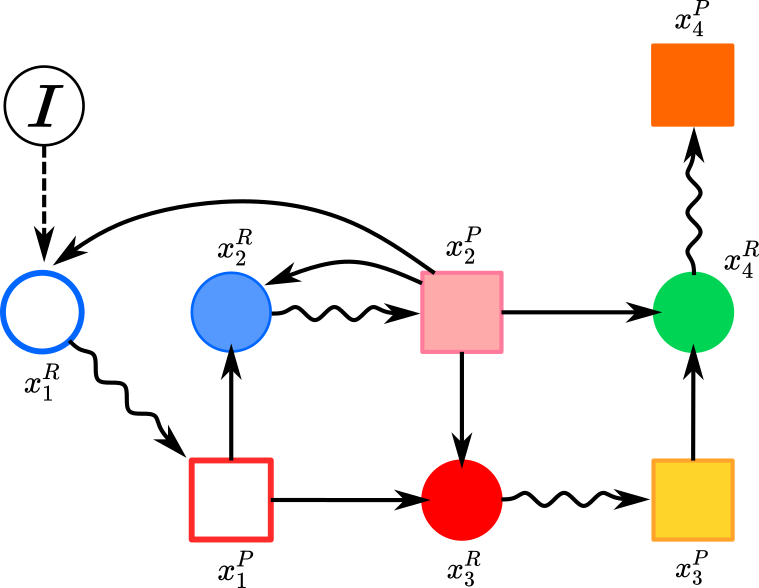
\includegraphics[scale=0.6]{figs/broken_fibo_2.png}
    \caption{Fibonacci circuit $\varphi_2$ with input node $x_1^R$ and output node $x_4^P$.}
    \label{fig:x1input_fibo}    
\end{figure}

The special model \cite{stochs_gene_2005,homeostasis_antonelli2018} used for this circuit is given by the set 
of nonlinear differential equations of Eq.~\ref{eq:special_fibo1}:
\begin{equation} \label{eq:special_fibo1}
    \begin{aligned} f_{x_1^R}(x_1^R, x_2^P, \mathcal{I}) &= -\delta x_1^R + \gamma\tilde{f}(x_2^P) + \mathcal{I}\\ 
        f_{x_1^P}(x_1^P, x_1^R) &= -\alpha x_1^P + \beta x_1^R \\ 
        f_{x_2^R}(x_2^R, x_1^P, x_2^P) &= -\delta x_2^R + \gamma\tilde{g}(x_1^P, x_2^P) \\ 
        f_{x_2^P}(x_2^P, x_2^R) &= -\alpha x_2^P + \beta x_2^R   \\ 
        f_{x_3^R}(x_3^R, x_1^P, x_2^P) &= -\delta x_3^R + \gamma \tilde{g}(x_1^P,x_2^P) \\ 
        f_{x_3^P}(x_3^P, x_3^R) &= -\alpha x_3^P + \beta x_3^R \\ 
        f_{x_4^R}(x_4^R, x_2^P, x_3^P) &= -\delta x_4^R + \gamma \tilde{h}(x_2^P, x_3^P) \\ 
        f_{x_4^P}(x_4^P, x_4^R) &= -\alpha x_4^P + \beta x_4^R
    \end{aligned},
\end{equation}
where $\tilde{f}$, $\tilde{g}$ and $\tilde{h}$ are monotonic nonlinear functions within the interval $[0,1]$. 
Specifically, $\tilde{f}$, $\tilde{g}$ and $\tilde{h}$ are defined as Hill functions,
with $\tilde{g}(x_1^P, x_2^P) = \tilde{g}(x_1^P + x_2^P)$ and $\tilde{h}(x_2^P, x_3^P) = \tilde{h}(x_2^P + x_3^P)$.
For this circuit, we are imposing the restriction that the input function of $x_2^R$ and $x_3^R$ are given 
by the same function $\tilde{g}(x_1^P, x_2^P)$ which is motivated by the Fibonacci circuit realization in 
\textit{E. Coli} gene network where all regulations within the fiber are repressors \cite{morone2020}.

Using the algorithm of \cite{wang2021}, we obtain the general infinitesimal homeostasis condition at 
point $\mathcal{I}_0$ for this input-output network according to the special model of 
Eq.~\ref{eq:special_fibo1}:
\begin{equation} \label{eq:special_infhom_fibo}
    2\alpha\delta\gamma^2\beta\tilde{g}'(x_1^P + x_2^P)\tilde{h}'(x_2^P + x_3^P) = 0.
\end{equation} 

Considering the condition of Eq.~\ref{eq:special_infhom_fibo}, we can determine the relations 
to be satisfied together with the additional conditions for infinitesimal chair at $\mathcal{I}_0$. 
However, because of the simple form of Eq.~\ref{eq:special_infhom_fibo},
we only state the condition of infinitesimal homeostasis, $x_{4(\infty), \mathcal{I}}^P(\mathcal{I}_0) = 0$, 
for a given stable equilibrium $\vec{x}_{\infty}$ at $\mathcal{I}_0$, as
\begin{equation}
    \rho(\mathcal{I}_0) \equiv \tilde{g}(x_1^P, x_2^P)\tilde{h}(x_2^P,x_3^P) = \tilde{g}(x_1^P +  x_2^P)\tilde{h}(x_2^P + x_3^P) = 0, 
\end{equation}
which can only be satisfied for two cases: total degradation of the protein concentration
($x_{1,2}^P(\mathcal{I}) +  x_{2,3}^P(\mathcal{I}) = 0$), or saturation 
of these same quantities: $x_{1,2}^P(\mathcal{I}) +  x_{2,3}^P(\mathcal{I}) \rightarrow \infty$, 
where $\infty$ only means that the sum is large enough to satisfy either 
$\tilde{g}' = 0$ or $\tilde{h}' = 0$. Furthermore, by considering only these two possibilities
we have that all the other higher-order derivatives also approach zero for those cases. We can 
observe the specifics of this type of behavior in the numerical example of Fig.~\ref{fig:fibo_x1r_ex1}.



\begin{figure}[H]
    \centering
    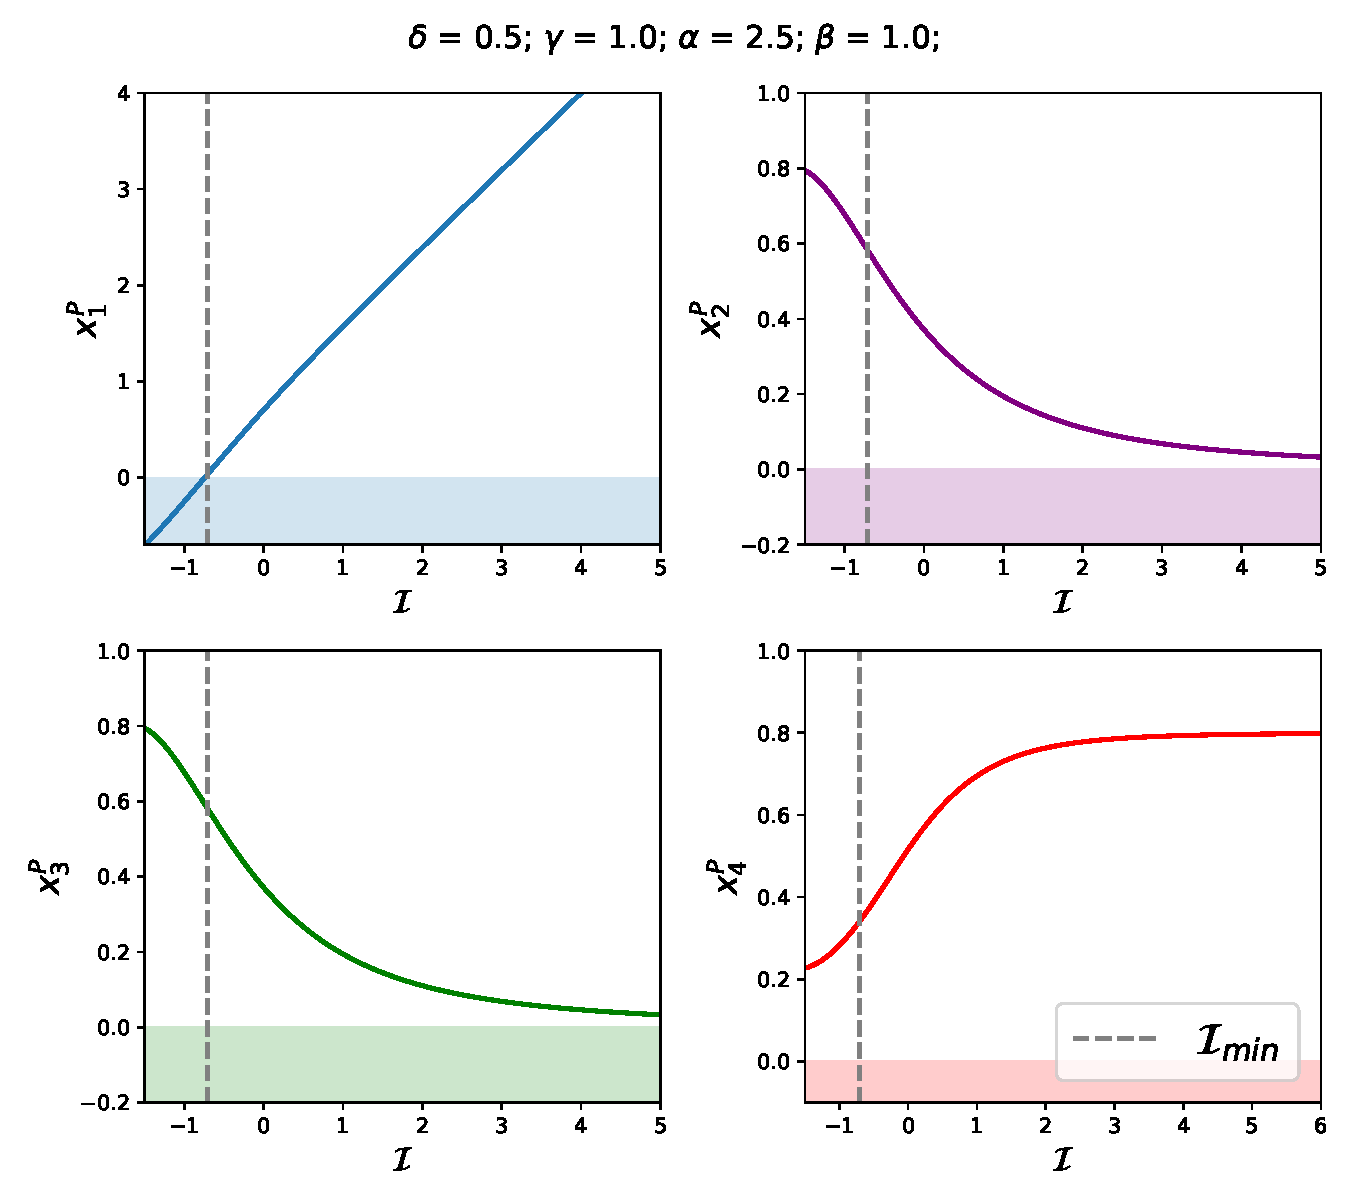
\includegraphics[scale=0.52]{figs/numerics/fibo_x1r_ex1.pdf}
    \caption{Protein concentrations for the Fibonacci circuit with input node $x_1^R$.
    By adding the input to $x_1^R$, the fibration symmetry is preserved and the concentrations
    of $x_2^P$ and $x_3^P$ are synchronized.}
    \label{fig:fibo_x1r_ex1}
\end{figure}

\subsection{Input node $x_2^R$}

The diagram of this circuit is shown at Fig.~\ref{fig:x2input_fibo}.

\begin{figure}[H]
    \centering
    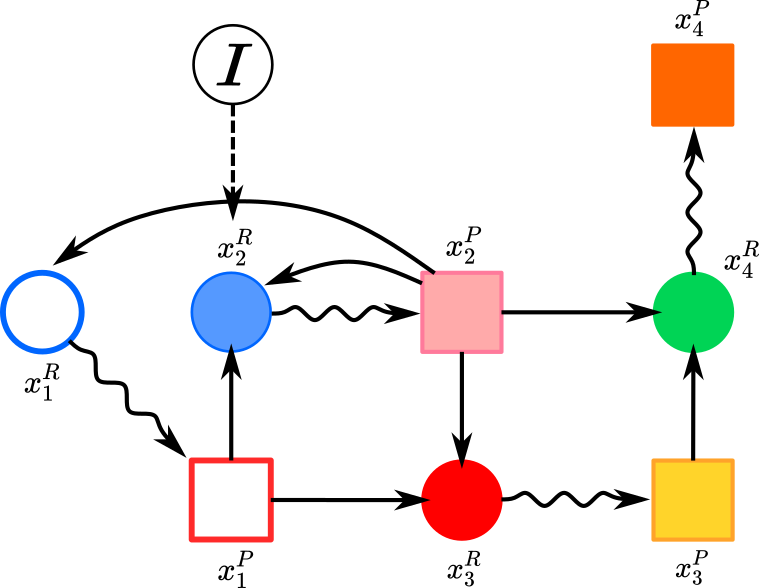
\includegraphics[scale=0.6]{figs/broken_fibo_1.png}
    \caption{Fibonacci circuit $\varphi_2$ with input node $x_2^R$ and output node $x_4^P$.}
    \label{fig:x2input_fibo}    
\end{figure}

The special model \cite{stochs_gene_2005,homeostasis_antonelli2018} used for this circuit is given by the set 
of nonlinear differential equations of Eq.~\ref{eq:special_fibo2}:
\begin{equation} \label{eq:special_fibo2}
    \begin{aligned} 
        f_{x_1^R}(x_1^R, x_2^P) &= -\delta x_1^R + \gamma\tilde{f}(x_2^P) \\ 
        f_{x_1^P}(x_1^P, x_1^R) &= -\alpha x_1^P + \beta x_1^R \\ 
        f_{x_2^R}(x_2^R, x_1^P, x_2^P, \mathcal{I}) &= -\delta x_2^R + \gamma\tilde{g}(x_1^P, x_2^P) + \mathcal{I} \\ 
        f_{x_2^P}(x_2^P, x_2^R) &= -\alpha x_2^P + \beta x_2^R   \\ 
        f_{x_3^R}(x_3^R, x_1^P, x_2^P) &= -\delta x_3^R + \gamma \tilde{g}(x_1^P,x_2^P) \\ 
        f_{x_3^P}(x_3^P, x_3^R) &= -\alpha x_3^P + \beta x_3^R \\ 
        f_{x_4^R}(x_4^R, x_2^P, x_3^P) &= -\delta x_4^R + \gamma \tilde{h}(x_2^P, x_3^P) \\ 
        f_{x_4^P}(x_4^P, x_4^R) &= -\alpha x_4^P + \beta x_4^R
    \end{aligned}
\end{equation}
where $\tilde{f}$, $\tilde{g}$ and $\tilde{h}$ are monotonic nonlinear functions within the interval $[0,1]$. 
Specifically, $\tilde{f}$, $\tilde{g}$ and $\tilde{h}$ are defined as Hill functions,
with $\tilde{g}(x_1^P, x_2^P) = \tilde{g}(x_1^P + x_2^P)$ and $\tilde{h}(x_2^P, x_3^P) = \tilde{h}(x_2^P + x_3^P)$.
Following the same motivation of the previous circuit in subsection~\ref{ssec:fibo_x1}, we impose 
that the input function of $x_2^R$ and $x_3^R$ are given by the same function $\tilde{g}(x_1^P, x_2^P)$,
according to what is observed in the gene network of \textit{E. Coli} \cite{morone2020}.

Using the algorithm of \cite{wang2021}, we obtain the infinitesimal homeostasis condition at  
$\mathcal{I}_0$ for this particular input-output network according to the special model in 
Eq.~\ref{eq:special_fibo2}. Therefore, we can state that at a given stable equilibrium $\vec{x}_{(\infty)}$
the infinitesimal homeostasis condition, $x_{4(\infty), \mathcal{I}}^P(\mathcal{I}_0) = 0$, is satisfied iff:
\begin{equation} \label{eq:special_infhom_fibo2}
    \rho(\mathcal{I}_0) \equiv \tilde{h}'(x_2^P, x_3^P)\bigg[ \delta^2\alpha^2 + \delta\alpha\beta\gamma\tilde{g}'(x_1^P, x_2^P) + \gamma^2\beta^2\tilde{f}'(x_2^P)\tilde{g}'(x_1^P, x_2^P)\bigg] = 0.
\end{equation} 
This condition implies the additional conditions
\begin{equation}
    \frac{d\rho}{d\mathcal{I}}(\mathcal{I}_0) = 0 \ \ \text{ and } \ \ \frac{d^2\rho}{d\mathcal{I}^2}(\mathcal{I}_0) \neq 0
\end{equation}
for the infinitesimal chair condition.

Therefore, to satisfy Eq.~\ref{eq:special_infhom_fibo2} we have two possibilities: either 
the first term or the second term is zero at $\mathcal{I}_0$. The first scenario occurs only for 
$x_2^P(\mathcal{I}) + x_3^P(\mathcal{I}) = 0$ and
$x_2^P(\mathcal{I}) + x_3^P(\mathcal{I}) \rightarrow \infty$, where $\infty$ here only 
means that the sum is large enough to satisfy the condition.  Although this scenario is possible 
(as observed in the SAT-FFF), we consider only the second scenario, since it might 
provide more nontrivial homeostatic mechanisms.

Thus, by considering the four general condition for an infinitesimal chair point 
(equilibrium, $\rho(\mathcal{I}_0) = 0$, $\rho_{\mathcal{I}}(\mathcal{I}_0) = 0$ and 
$\rho_{\mathcal{II}}(\mathcal{I}_0) \neq 0$), we obtain the following relations:
\begin{equation}
    \tilde{g}(x_1^P + x_2^P) = \frac{\alpha\delta}{\beta\gamma}x_2^P - \frac{\mathcal{I}}{\gamma},
\end{equation}
from the equilibrium condition. For $\rho(\mathcal{I}_0) = 0$, we have 
\begin{equation}
    \tilde{g}'(x_1^P + x_2^P) = - \frac{\alpha^2\delta^2}{\alpha\delta\beta\gamma + \gamma^2\beta^2\tilde{f}'(x_2^P)}.
\end{equation}
Moreover, for $\rho_{\mathcal{I}}(\mathcal{I}_0) = 0$ and 
$\rho_{\mathcal{II}}(\mathcal{I}_0) \neq 0$, we obtain
\begin{equation} \label{eq:chair1-fibo-x2r}
    \begin{split} 
        &{g}''(x_1^P + x_2^P)(x_{1,\mathcal{I}}^P + x_{2,\mathcal{I}}^P) \bigg[ \alpha\delta\beta\gamma + \gamma^2\beta^2\tilde{f}'(x_2^P)\bigg] \\ 
        & + \gamma^2\beta^2\tilde{g}'(x_1^P + x_2^P)\tilde{f}''(x_2^P)x_{2,\mathcal{I}}^P = 0 
    \end{split},
\end{equation}
and
\begin{equation}
    \begin{split} 
        \bigg\{ \tilde{g}'''(x_1^P + x_2^P)&(x_{1,\mathcal{I}}^P + x_{2,\mathcal{I}}^P)^2 \Big[\alpha\delta\beta\gamma + \gamma^2\beta^2\tilde{f}'(x_2^P)\Big] \\ 
        & + \gamma^2\beta^2\tilde{f}'''(x_2^P)\tilde{g}'(x_1^P + x_2^P)(x_{2,\mathcal{I}}^P)^2 \bigg\} \neq 0 
    \end{split},
\end{equation}
respectively.

\subsubsection{Key quantities}

To perform the next calculations we assume that $\tilde{g}''(x_1^P + x_2^P) = 0$ and $\tilde{f}''(x_2^P) = 0$, 
such that Eq.~\ref{eq:chair1-fibo-x2r} for $\rho_{\mathcal{I}}(\mathcal{I}_0)$ is satisfied. Therefore, we work
on four cases regarding the combinations of the regulations $\tilde{f}$ and $\tilde{g}$. Before introducing 
these specific cases, let us calculate the main quantities to be used later.

Whether $\tilde{f} \equiv S$ or $\tilde{f} \equiv 1 - S$, we obtain $x_{2(\infty)}^P = \pm 1/\sqrt{3}$ for the 
protein concentration $x_2^P$ at equilibrium satisfying the partial chair condition $\tilde{f}''(x_2^P) = 0$, 
while from $\tilde{g}''(x_1^P + x_2^P) = 0$ we have either $x_{1(\infty)}^P = 0$ or 
$x_{1,(\infty)}^P = \mp 2/\sqrt{3}$ for protein concentration $x_1^P$. This way, we have the following 
combinations for the concentrations $x_1^P$ and $x_2^P$ at homeostasis point:
\begin{equation}
    \begin{aligned}
        x_{1,(\infty)}^P = 0 \ \ \text{and} \ \ x_{2,(\infty)}^P = \pm \frac{1}{\sqrt{3}}\\
        x_{1,(\infty)}^P = \mp \frac{2}{\sqrt{3}} \ \ \text{and} \ \ x_{2,(\infty)}^P = \pm \frac{1}{\sqrt{3}}
    \end{aligned},
\end{equation}
giving a total four combinations for the concentrations $x_1^P$ and $x_2^P$ at the homeostasis point. We note 
that from these four combinations, only one provides a realistic scenario, since it does not predict negative
concentrations either for $x_1^P$ or $x_2^P$.

Moreover, we calculate key quantities useful for the analysis of specific cases. First, regarding the first 
derivatives of $\tilde{f}$:
\begin{equation}
    \begin{aligned}
        \tilde{f}'\Big(x_{2,(\infty)}^P &= \pm \frac{1}{\sqrt{3}}\Big) = \mp \frac{3\sqrt{3}}{8} \ \ (\tilde{f} \equiv S)\\
        \tilde{f}'\Big(x_{2,(\infty)}^P &= \pm \frac{1}{\sqrt{3}}\Big) = \pm \frac{3\sqrt{3}}{8} \ \ (\tilde{f} \equiv 1 - S)\\
    \end{aligned}.
\end{equation}
Now for $\tilde{g}$ and its first derivative. For $\tilde{g} \equiv S$, we have:
\begin{equation}
    \begin{aligned}
        &\tilde{g}(x_{1,(\infty)}^P + x_{2,(\infty)}^P) = \frac{3}{4}\\
        &\tilde{g}'\Big(x_{1,(\infty)}^P = 0, x_{2,(\infty)}^P = \pm \frac{1}{\sqrt{3}}\Big) = \mp \frac{3\sqrt{3}}{8} \\
        &\tilde{g}'\Big(x_{1,(\infty)}^P = \mp\frac{2}{\sqrt{3}}, x_{2,(\infty)}^P = \pm \frac{1}{\sqrt{3}}\Big) = \pm \frac{3\sqrt{3}}{8}\\
        &\mathcal{I}_0 = \gamma\bigg[ \frac{\alpha\delta}{\beta\gamma}x_{2,(\infty)}^P - \frac{3}{4} \bigg], \ \ \ \text{for} \ \ \ x_{2,(\infty)}^P = \pm\frac{1}{\sqrt{3}}
    \end{aligned},
\end{equation}
and for $\tilde{g} \equiv 1 - S$:
\begin{equation}
    \begin{aligned}
        &\tilde{g}(x_{1,(\infty)}^P + x_{2,(\infty)}^P) = \frac{1}{4}\\
        &\tilde{g}'(x_{1(\infty)}^P = 0, \ x_{2(\infty)}^P = \pm 1/\sqrt{3}) = \pm \frac{3\sqrt{3}}{8} \\
        &\tilde{g}'(x_{1(\infty)}^P = \mp 2/\sqrt{3}, \ x_{2(\infty)}^P = \pm 1/\sqrt{3}) = \mp \frac{3\sqrt{3}}{8} \\
        &\mathcal{I}_0 = \gamma\bigg[ \frac{\alpha\delta}{\beta\gamma}x_{2,(\infty)}^P - \frac{1}{4} \bigg], \ \ \ \text{for} \ \ \ x_{2,(\infty)}^P = \pm\frac{1}{\sqrt{3}}
    \end{aligned}
\end{equation}


\subsubsection{Case 1: $\tilde{f}(x_2^P) \equiv S(x_2^P)$ and $\tilde{g}(x_1^P + x_2^P) \equiv S(x_1^P + x_2^P)$}

Define $D = 3\sqrt{3}/8$. For $x_{1,(\infty)}^P = 0$ and $x_{2,(\infty)}^P = \pm 1/\sqrt{3}$ we obtain,
 from Eq.~\ref{eq:chair1-fibo-x2r}, 
\begin{equation}
    D^2\bigg(\frac{\gamma\beta}{\alpha\delta}\bigg)^2 \mp D\frac{\gamma\beta}{\alpha\delta} + 1 = 0,
\end{equation}
which results only in complex values of $\gamma\beta/\alpha\delta$. This case is discarded for further analysis.

For $x_{1,(\infty)}^P = \mp 2/\sqrt{3}$ and $x_{2,(\infty)}^P = \pm 1/\sqrt{3}$ we obtain
\begin{equation}
    -D^2\bigg(\frac{\gamma\beta}{\alpha\delta}\bigg)^2 \pm D\frac{\gamma\beta}{\alpha\delta} + 1 = 0,
\end{equation}
which results in real values of $\gamma\beta/\alpha\delta$. More specifically, we have 
\begin{equation} \label{eq:case1-parameters}
    \frac{\gamma\beta}{\alpha\delta} = \frac{4}{9}\bigg[ \pm \sqrt{3} \mp^{root} \sqrt{15} \bigg],
\end{equation}
where $\mp^{root}$ is independent of the signs of $x_1^P$ and $x_2^P$ at the equilibrium. Then,
considering the Eq.~\ref{eq:case1-parameters} above, we have two main scenarios:
\begin{equation}
    \frac{\gamma\beta}{\alpha\delta} = \frac{4}{9}\bigg[ + \sqrt{3} \mp^{root} \sqrt{15} \bigg],
\end{equation} 
and 
\begin{equation}
    \frac{\gamma\beta}{\alpha\delta} = \frac{4}{9}\bigg[ - \sqrt{3} \mp^{root} \sqrt{15} \bigg],
\end{equation}
each one related to one combination between the values of $x_{1,(\infty)}^P$ and $x_{2,(\infty)}^P$.
From the assumptions that all model parameters are nonnegative, we only consider the cases where $\mp^{root}$
leads to $\gamma\beta/\alpha\delta > 0$. Since here both situations leads to one negative protein 
concentration, we only consider $x_{1,(\infty)}^P = + 2/\sqrt{3}$ and $x_{2,(\infty)}^P = - 1/\sqrt{3}$
to display the chair behavior around $\mathcal{I}_0$. Therefore, for $\gamma\beta/\alpha\delta > 0$,
we have 
\begin{equation}
    \frac{\gamma\beta}{\alpha\delta} = \frac{4}{9}\bigg[ - \sqrt{3} + \sqrt{15} \bigg],
\end{equation}
and 
\begin{equation}
    \mathcal{I}_0 = -\gamma \bigg(\frac{\alpha\delta}{\beta\gamma}\frac{1}{\sqrt{3}} + \frac{3}{4}\bigg),
\end{equation}
allowing us to obtain the chair behavior shown at Fig.~\ref{fig:case1-fibo-chair}.

\begin{figure}[H]
    \centering
    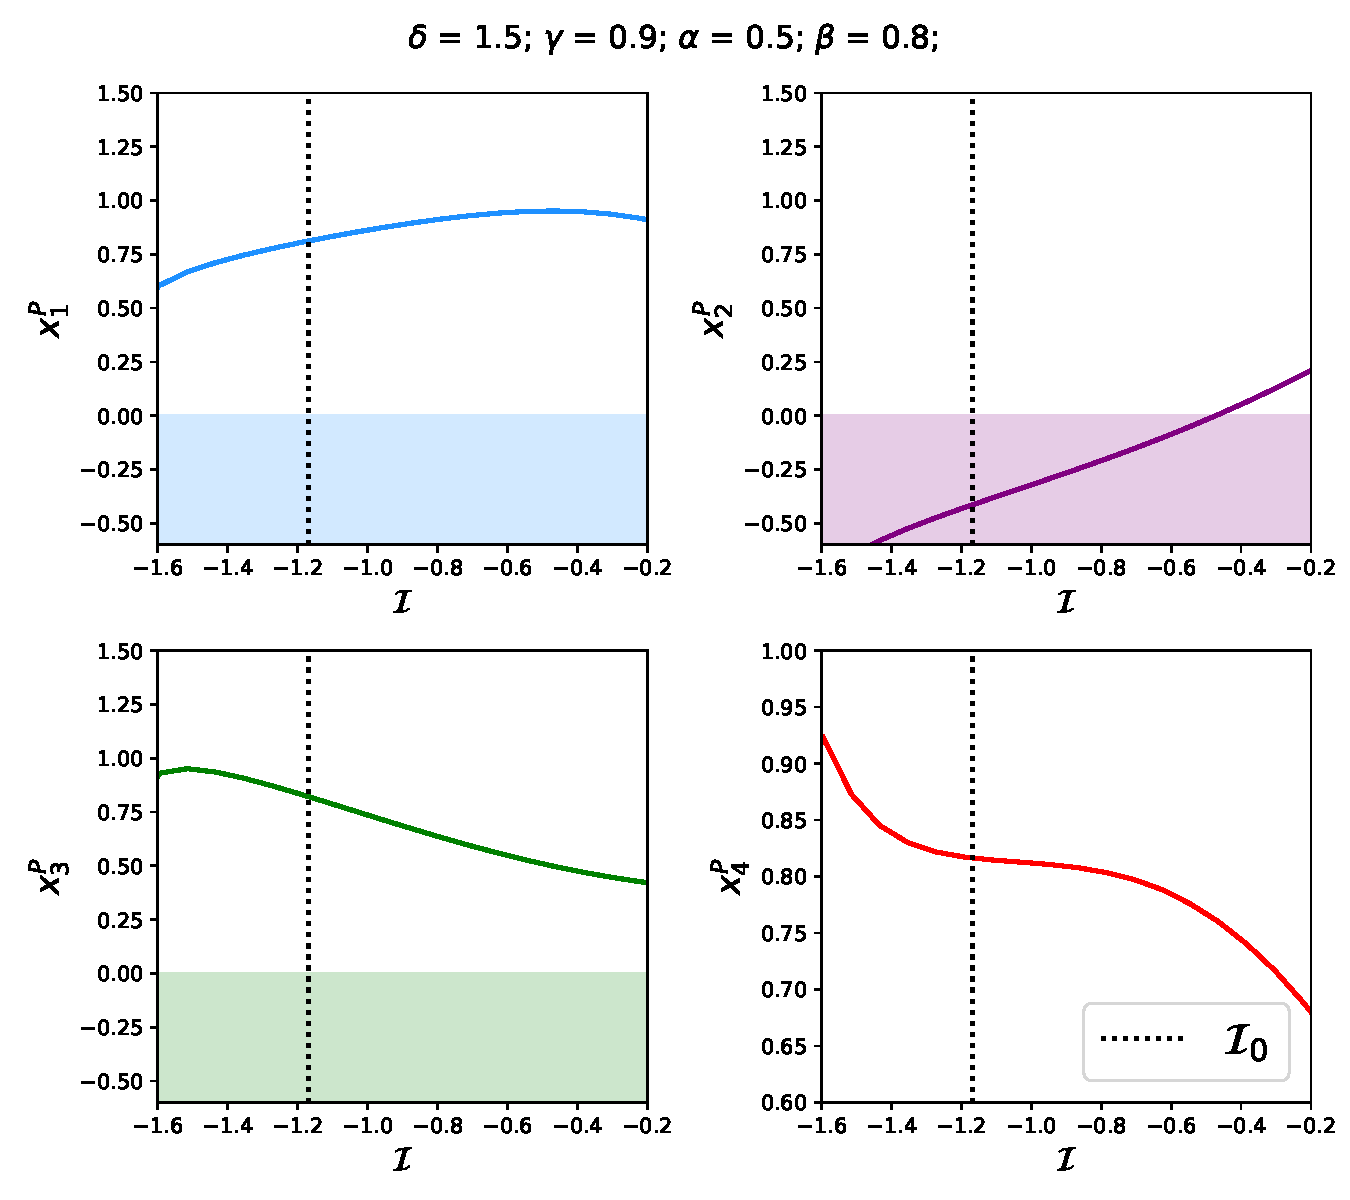
\includegraphics[scale=0.5]{figs/numerics/fibo_x2r_case1.pdf}
    \caption{Protein concentrations for the Fibonacci circuit with input node $x_2^R$.}
    \label{fig:case1-fibo-chair}
\end{figure}

\subsubsection{Case 2: $\tilde{f}(x_2^P) \equiv 1 - S(x_2^P)$ and $\tilde{g}(x_1^P + x_2^P) \equiv S(x_1^P + x_2^P)$}

Define $D = 3\sqrt{3}/8$. For $x_{1,(\infty)}^P = \mp 2/\sqrt{3}$ and $x_{2,(\infty)}^P = \pm 1/\sqrt{3}$ we obtain,
 from Eq.~\ref{eq:chair1-fibo-x2r},  
\begin{equation}
    D^2\bigg(\frac{\gamma\beta}{\alpha\delta}\bigg)^2 \pm D\frac{\gamma\beta}{\alpha\delta} + 1 = 0,
\end{equation}
which results only in complex values of $\gamma\beta/\alpha\delta$. This case is discarded for further analysis.

For $x_{1,(\infty)}^P = 0$ and $x_{2,(\infty)}^P = \pm 1/\sqrt{3}$ we obtain 
\begin{equation}
    -D^2\bigg(\frac{\gamma\beta}{\alpha\delta}\bigg)^2 \mp D\frac{\gamma\beta}{\alpha\delta} + 1 = 0,
\end{equation}
which results in real values of $\gamma\beta/\alpha\delta$. More specifically, we have 
\begin{equation} \label{eq:case2-parameters}
    \frac{\gamma\beta}{\alpha\delta} = \frac{4}{9}\bigg[ \mp \sqrt{3} \mp^{root} \sqrt{15} \bigg],
\end{equation}
where $\mp^{root}$ is independent of the signs of $x_1^P$ and $x_2^P$ at the equilibrium. Then,
considering the Eq.~\ref{eq:case2-parameters} above, we have two main scenarios:
\begin{equation}
    \frac{\gamma\beta}{\alpha\delta} = \frac{4}{9}\bigg[ - \sqrt{3} \mp^{root} \sqrt{15} \bigg],
\end{equation} 
and 
\begin{equation}
    \frac{\gamma\beta}{\alpha\delta} = \frac{4}{9}\bigg[ + \sqrt{3} \mp^{root} \sqrt{15} \bigg],
\end{equation}
each one related to one combination between the values of $x_{1,(\infty)}^P$ and $x_{2,(\infty)}^P$.
Again, we only consider the cases where $\mp^{root}$ leads to $\gamma\beta/\alpha\delta > 0$. Here, 
there is one combination for which both concentrations $x_{1,(\infty)}^P$ and $x_{2,(\infty)}^P$ are 
nonnegative, and we consider this case to display the chair behavior around $\mathcal{I}_0$. Therefore, 
for $\gamma\beta/\alpha\delta > 0$, we have 
\begin{equation}
    \frac{\gamma\beta}{\alpha\delta} = \frac{4}{9}\bigg[ - \sqrt{3} + \sqrt{15} \bigg],
\end{equation}
and 
\begin{equation}
    \mathcal{I}_0 = \gamma \bigg(\frac{\alpha\delta}{\beta\gamma}\frac{1}{\sqrt{3}} - \frac{3}{4}\bigg),
\end{equation}
allowing us to obtain the chair behavior shown at Fig.~\ref{fig:case2-fibo-chair}.

\begin{figure}[H]
    \centering
    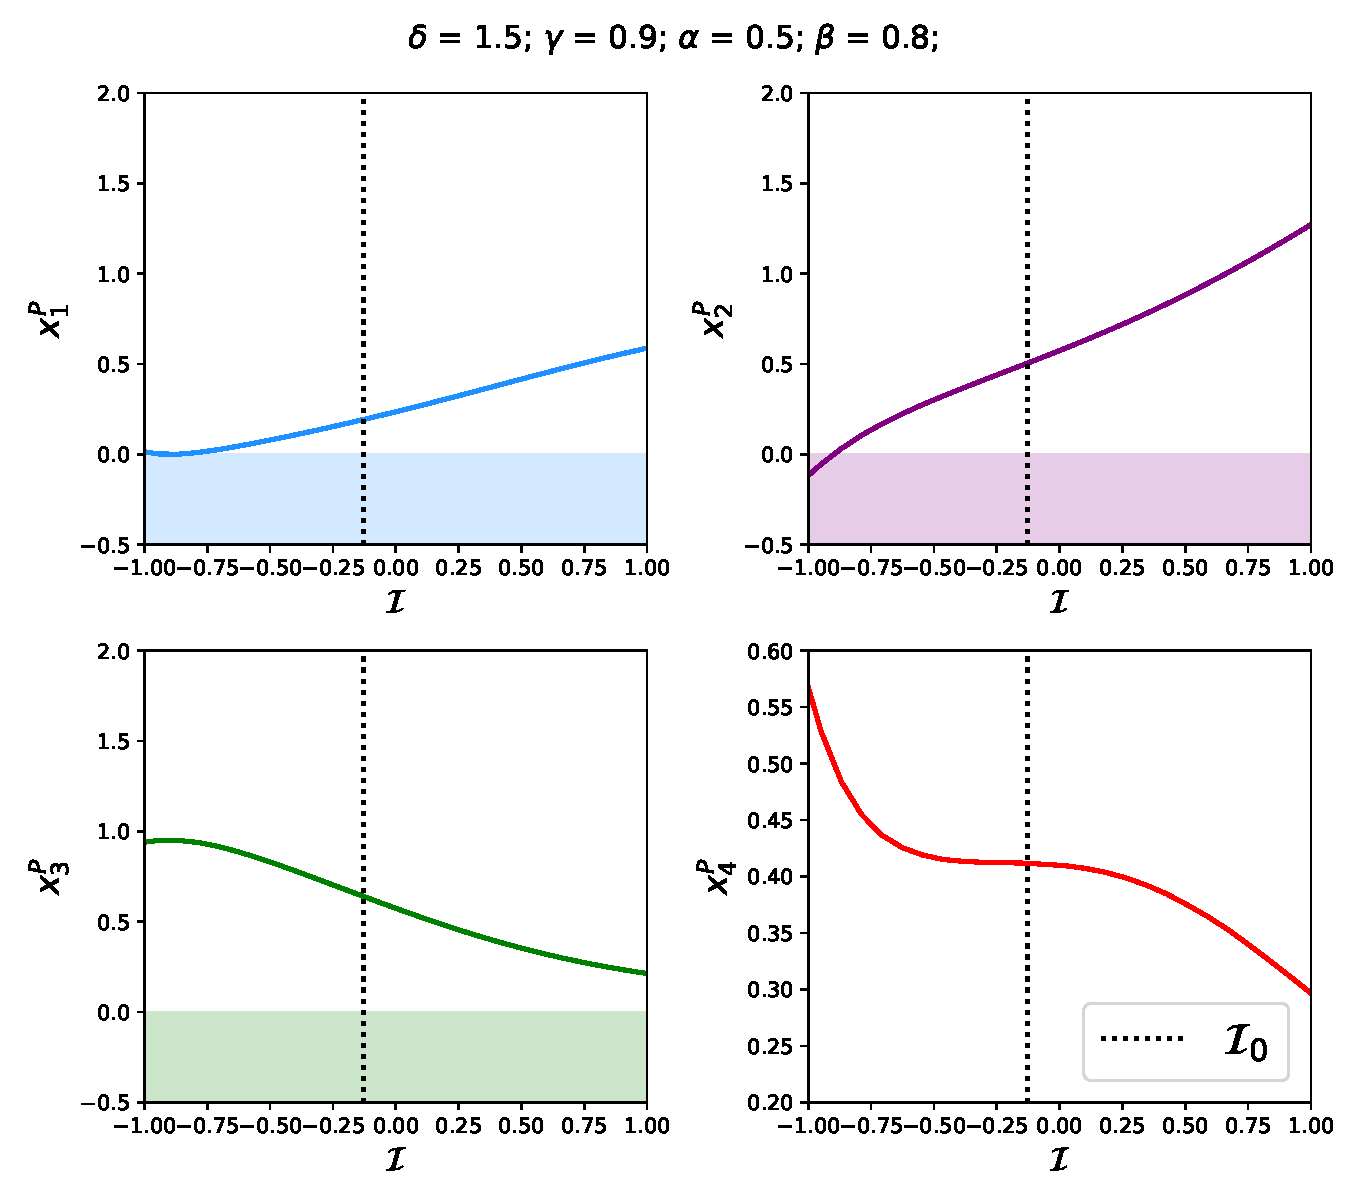
\includegraphics[scale=0.5]{figs/numerics/fibo_x2r_case2.pdf}
    \caption{Protein concentrations for the Fibonacci circuit with input node $x_2^R$.}
    \label{fig:case2-fibo-chair}
\end{figure}

\subsubsection{Case 3: $\tilde{f}(x_2^P) \equiv S(x_2^P)$ and $\tilde{g}(x_1^P + x_2^P) \equiv 1 - S(x_1^P + x_2^P)$}

Define $D = 3\sqrt{3}/8$. For $x_{1,(\infty)}^P = \mp 2/\sqrt{3}$ and $x_{2,(\infty)}^P = \pm 1/\sqrt{3}$ we obtain, 
from Eq.~\ref{eq:chair1-fibo-x2r},  
\begin{equation}
    D^2\bigg(\frac{\gamma\beta}{\alpha\delta}\bigg)^2 \mp D\frac{\gamma\beta}{\alpha\delta} + 1 = 0,
\end{equation}
which results only in complex values of $\gamma\beta/\alpha\delta$. This case is discarded for further analysis.

For $x_{1,(\infty)}^P = 0$ and $x_{2,(\infty)}^P = \pm 1/\sqrt{3}$ we obtain 
\begin{equation}
    -D^2\bigg(\frac{\gamma\beta}{\alpha\delta}\bigg)^2 \pm D\frac{\gamma\beta}{\alpha\delta} + 1 = 0,
\end{equation}
which results in real values of $\gamma\beta/\alpha\delta$. More specifically, we have 
\begin{equation} \label{eq:case3-parameters}
    \frac{\gamma\beta}{\alpha\delta} = \frac{4}{9}\bigg[ \pm \sqrt{3} \mp^{root} \sqrt{15} \bigg],
\end{equation}
where $\mp^{root}$ is independent of the signs of $x_1^P$ and $x_2^P$ at the equilibrium. Then,
considering the Eq.~\ref{eq:case3-parameters} above, we have two main scenarios:
\begin{equation}
    \frac{\gamma\beta}{\alpha\delta} = \frac{4}{9}\bigg[ + \sqrt{3} \mp^{root} \sqrt{15} \bigg],
\end{equation} 
and 
\begin{equation}
    \frac{\gamma\beta}{\alpha\delta} = \frac{4}{9}\bigg[ - \sqrt{3} \mp^{root} \sqrt{15} \bigg],
\end{equation}
each one related to one combination between the values of $x_{1,(\infty)}^P$ and $x_{2,(\infty)}^P$.
Considering the cases where $\mp^{root}$ leads to $\gamma\beta/\alpha\delta > 0$, we have
the combination for which both concentrations $x_{1,(\infty)}^P = 0$ and $x_{2,(\infty)}^P = +1/\sqrt{3}$ are 
nonnegative. We consider this case to display the homeostatic behavior around $\mathcal{I}_0$. Therefore, 
for $\gamma\beta/\alpha\delta > 0$, we have 
\begin{equation}
    \frac{\gamma\beta}{\alpha\delta} = \frac{4}{9}\bigg[ + \sqrt{3} + \sqrt{15} \bigg],
\end{equation}
and 
\begin{equation}
    \mathcal{I}_0 = \gamma \bigg(\frac{\alpha\delta}{\beta\gamma}\frac{1}{\sqrt{3}} - \frac{1}{4}\bigg),
\end{equation}
which are the estimated values for the case where the second term of the product 
of Eq.~\ref{eq:special_infhom_fibo2} is zero. However, as we observe in Fig.~\ref{fig:case3-fibo-chair}
this condition is not fulfilled. Instead, the circuit reaches homeostasis by saturation through
$\tilde{h}^{(n)}(x_2^P(\mathcal{I})+x_3^P(\mathcal{I})) \rightarrow 0$ as $\mathcal{I} > \mathcal{I}_c$
for some real value $\mathcal{I}_c$ and integer $n$ for high-order derivatives, as we can see 
in Fig.~\ref{fig:case3-fibo-hderivative}. Therefore, infinitesimal homeostasis $\rho(\mathcal{I}) = 0$
is satisfied by the vanishing of the first term of Eq.~\ref{eq:special_infhom_fibo2}.

\begin{figure}[H]
    \centering
    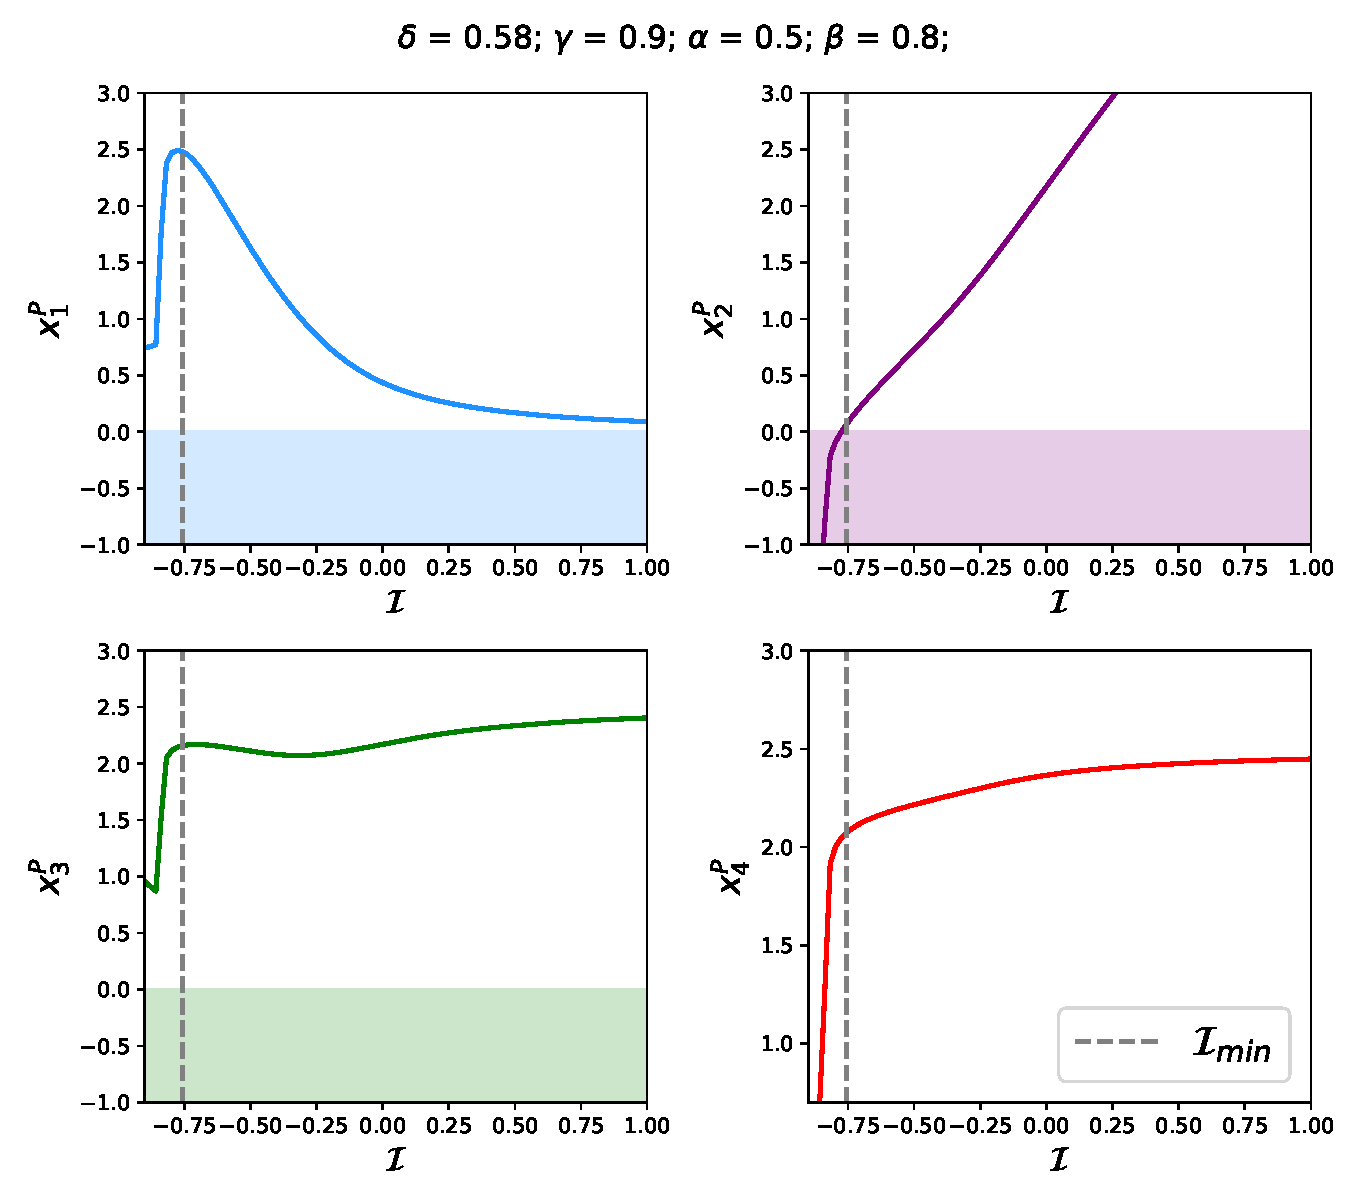
\includegraphics[scale=0.46]{figs/numerics/fibo_x2r_case3.pdf}
    \caption{Protein concentrations for the Fibonacci circuit with input node $x_2^R$.
    $\mathcal{I}_{min}$ is the minimum value of $\mathcal{I}$
    such that all protein concentrations are positive.}
    \label{fig:case3-fibo-chair}
\end{figure}

\begin{figure}[H]
    \centering
    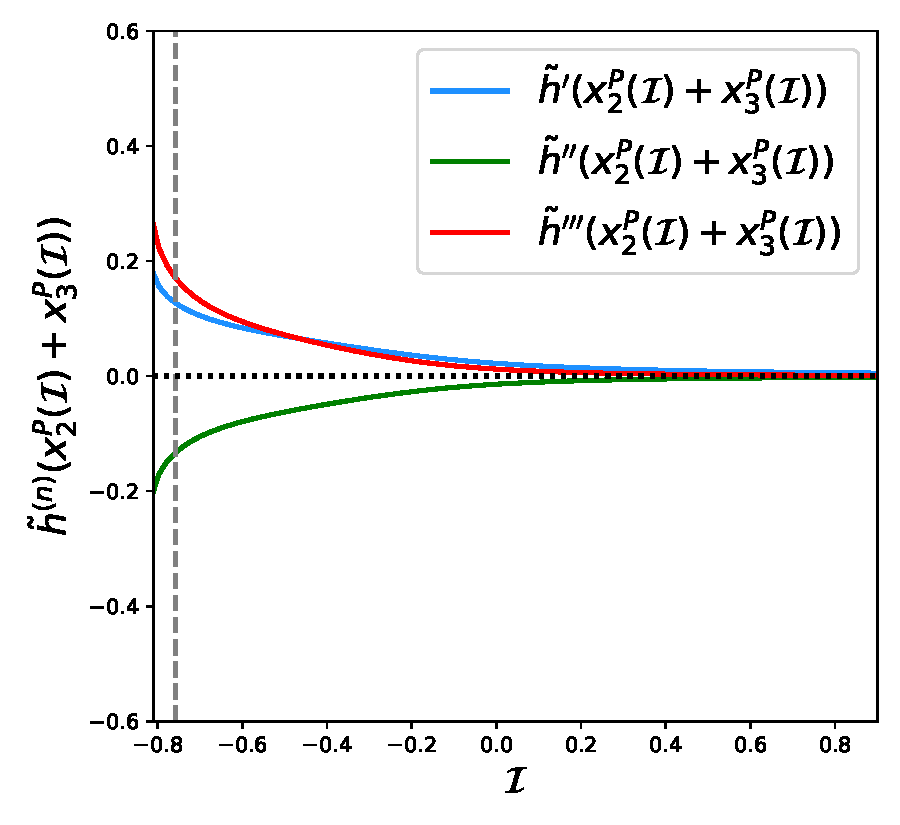
\includegraphics[scale=0.5]{figs/numerics/fibo_x2r_case3_h_derivative.pdf}
    \caption{Higher-order derivatives of $\tilde{h}(x_2^P + x_3^P)$ as functions of the input 
    parameter $\mathcal{I}$.}
    \label{fig:case3-fibo-hderivative}
\end{figure}

\subsubsection{Case 4: $\tilde{f}(x_2^P) \equiv 1 - S(x_2^P)$ and $\tilde{g}(x_1^P + x_2^P) \equiv 1 - S(x_1^P + x_2^P)$}

Define $D = 3\sqrt{3}/8$. For $x_{1,(\infty)}^P = 0$ and $x_{2,(\infty)}^P = \pm 1/\sqrt{3}$ we obtain,
 from Eq.~\ref{eq:chair1-fibo-x2r},  
\begin{equation}
    D^2\bigg(\frac{\gamma\beta}{\alpha\delta}\bigg)^2 \pm D\frac{\gamma\beta}{\alpha\delta} + 1 = 0,
\end{equation}
which results only in complex values of $\gamma\beta/\alpha\delta$. This case is discarded for further analysis.

For $x_{1,(\infty)}^P = \mp 2/\sqrt{3}$ and $x_{2,(\infty)}^P = \pm 1/\sqrt{3}$ we obtain 
\begin{equation}
    -D^2\bigg(\frac{\gamma\beta}{\alpha\delta}\bigg)^2 \mp D\frac{\gamma\beta}{\alpha\delta} + 1 = 0,
\end{equation}
which results in real values of $\gamma\beta/\alpha\delta$. More specifically, we have 
\begin{equation} \label{eq:case4-parameters}
    \frac{\gamma\beta}{\alpha\delta} = \frac{4}{9}\bigg[ \mp \sqrt{3} \mp^{root} \sqrt{15} \bigg],
\end{equation}
where $\mp^{root}$ is independent of the signs of $x_1^P$ and $x_2^P$ at the equilibrium. Then,
considering the Eq.~\ref{eq:case4-parameters} above, we have two main scenarios:
\begin{equation}
    \frac{\gamma\beta}{\alpha\delta} = \frac{4}{9}\bigg[ - \sqrt{3} \mp^{root} \sqrt{15} \bigg],
\end{equation} 
and 
\begin{equation}
    \frac{\gamma\beta}{\alpha\delta} = \frac{4}{9}\bigg[ + \sqrt{3} \mp^{root} \sqrt{15} \bigg],
\end{equation}
each one related to one combination between the values of $x_{1,(\infty)}^P$ and $x_{2,(\infty)}^P$.
Here we only consider the cases where $\gamma\beta/\alpha\delta > 0$. Also, since both situations 
satisfying $\gamma\beta/\alpha\delta > 0$ leads to one negative concentration we analyze the chair 
behavior only for the combination $x_{1,(\infty)}^P = + 2/\sqrt{3}$ and $x_{2,(\infty)}^P = - 1/\sqrt{3}$. 
Therefore,
\begin{equation}
    \frac{\gamma\beta}{\alpha\delta} = \frac{4}{9}\bigg[ + \sqrt{3} + \sqrt{15} \bigg],
\end{equation}
and 
\begin{equation}
    \mathcal{I}_0 = -\gamma \bigg(\frac{\alpha\delta}{\beta\gamma}\frac{1}{\sqrt{3}} + \frac{1}{4}\bigg),
\end{equation}
which are the estimated values for the case where the second term of the product 
of Eq.~\ref{eq:special_infhom_fibo2} is zero. Just like case 3, we observe in Fig.~\ref{fig:case4-fibo-chair}
that this condition is not fulfilled. Instead, the circuit reaches homeostasis again by saturation through
$\tilde{h}^{(n)}(x_2^P(\mathcal{I})+x_3^P(\mathcal{I})) \rightarrow 0$ as $\mathcal{I} > \mathcal{I}_c$
for some real value $\mathcal{I}_c$ and integer $n$ for high-order derivatives, as we can see 
in Fig.~\ref{fig:case4-fibo-hderivative}. Therefore, infinitesimal homeostasis $\rho(\mathcal{I}) = 0$
is satisfied by the vanishing of the first term of Eq.~\ref{eq:special_infhom_fibo2}. Furthermore, all the 
higher-order derivatives of $\tilde{h}$ also go to zero, satisfying all the higher derivatives $d^n\rho/d\mathcal{I}^n = 0$
and, thus, reaching a constant region for the input-output function $x_4^P(\mathcal{I})$.

\begin{figure}[H]
    \centering
    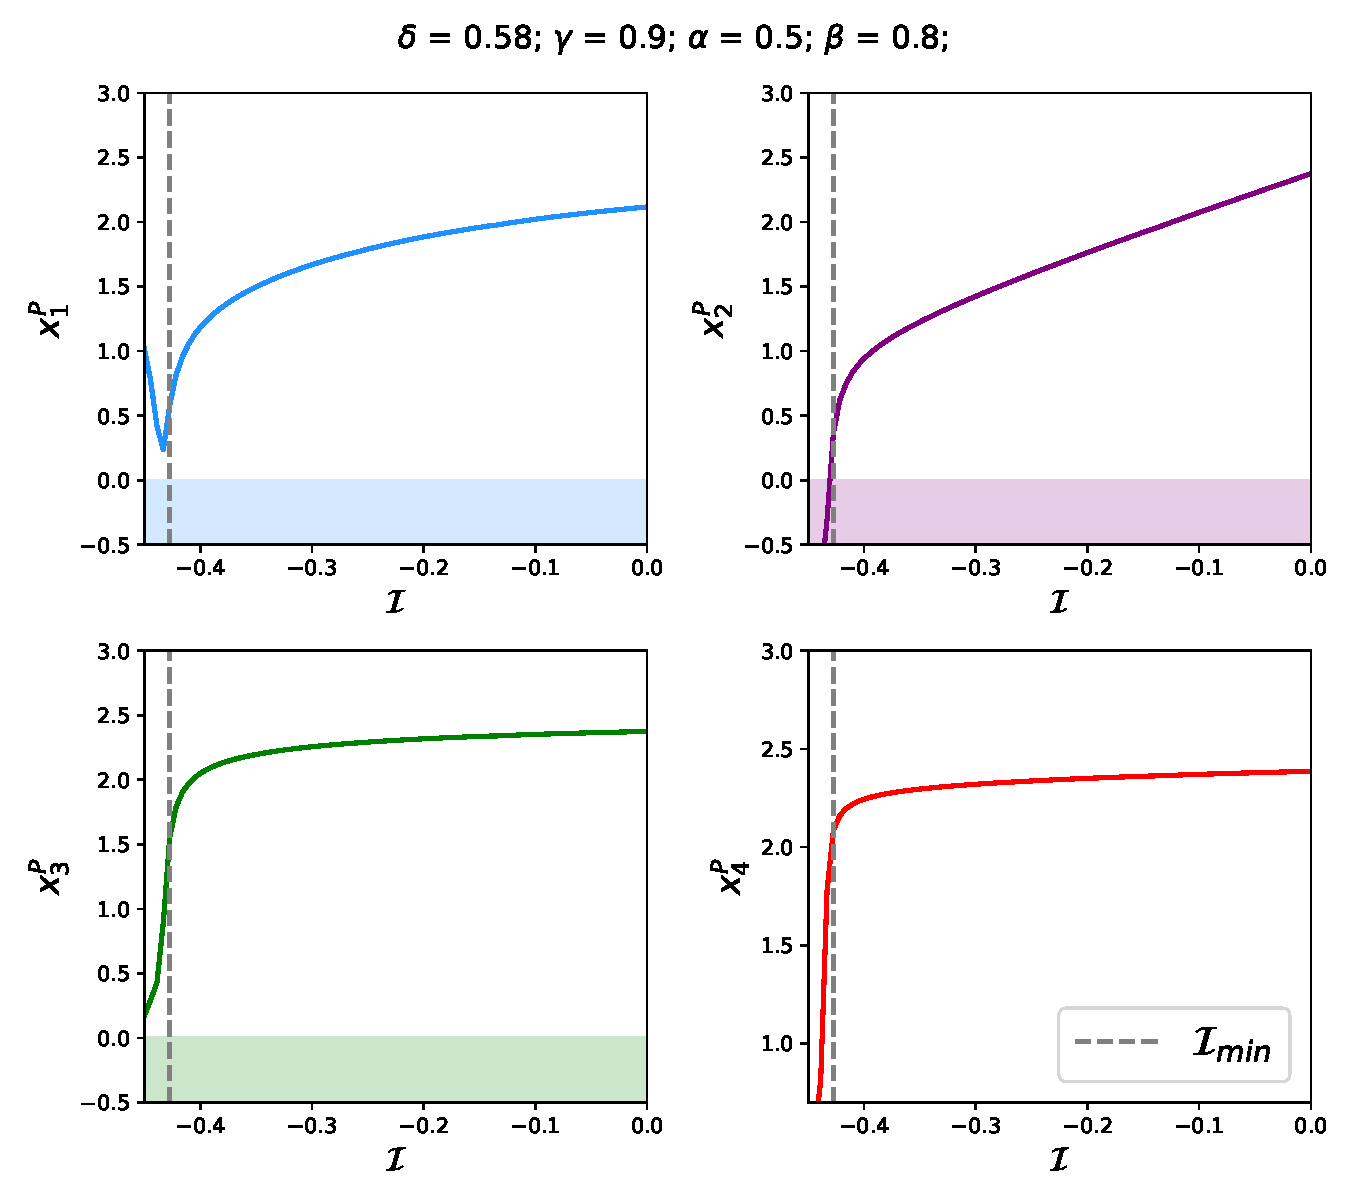
\includegraphics[scale=0.48]{figs/numerics/fibo_x2r_case4.pdf}
    \caption{Protein concentrations for the Fibonacci circuit with input node $x_2^R$. 
    $\mathcal{I}_{min}$ is the minimum value of $\mathcal{I}$ such that all protein 
    concentrations are positive.}
    \label{fig:case4-fibo-chair}
\end{figure}

\begin{figure}[H]
    \centering
    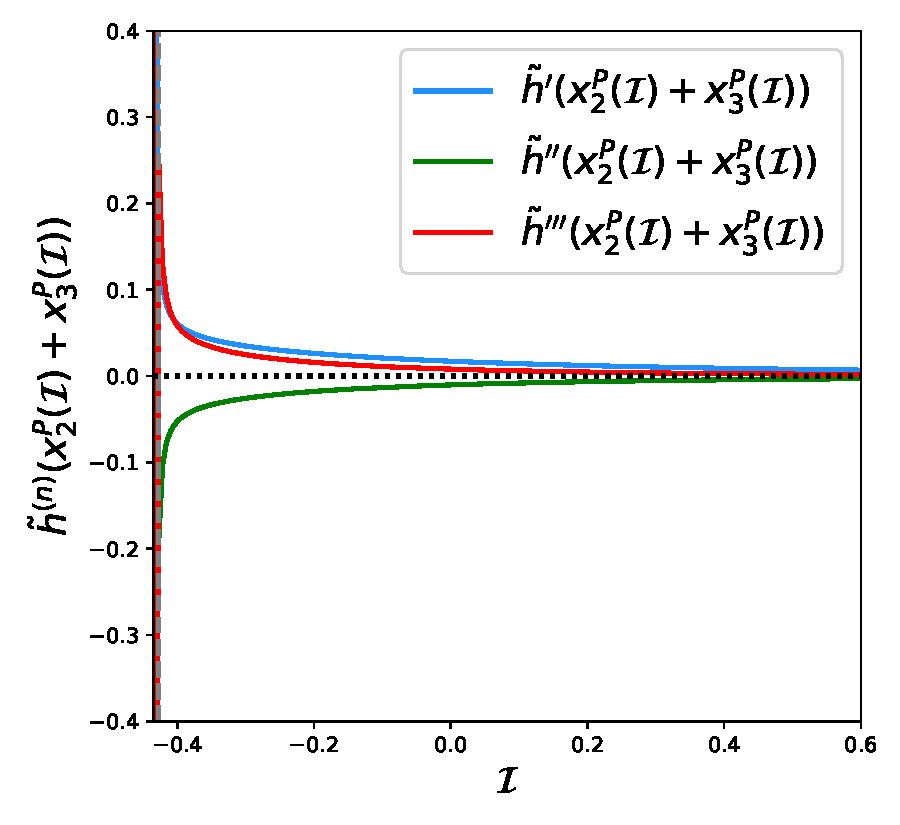
\includegraphics[scale=0.5]{figs/numerics/fibo_x2r_case4_h_derivative.pdf}
    \caption{Higher-order derivatives of $\tilde{h}(x_2^P + x_3^P)$ as functions of the input 
    parameter $\mathcal{I}$.}
    \label{fig:case4-fibo-hderivative}
\end{figure}